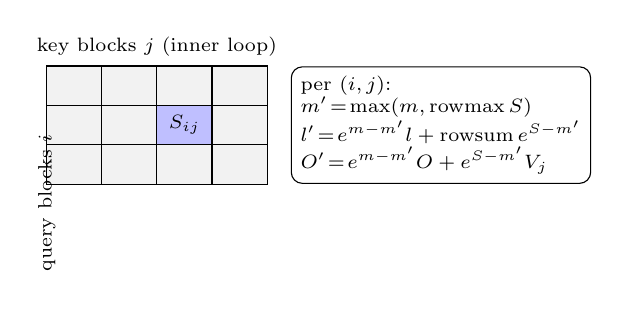
\begin{tikzpicture}[font=\scriptsize]
\foreach \i in {0,1,2} \foreach \j in {0,1,2,3} {
  \draw[fill=gray!10] (\j*0.7,-\i*0.5) rectangle ++(0.7,-0.5);
}
\draw[fill=blue!25] (1.4,-0.5) rectangle ++(0.7,-0.5);
\node at (1.75,-0.75) {$S_{ij}$};
\node[above] at (1.4,0) {key blocks $j$ (inner loop)};
\node[rotate=90,left] at (0,-0.75) {query blocks $i$};
\node[draw,rounded corners,align=left,right] at (3.1,-0.75) {per $(i,j)$:\\ $m'\!=\!\max(m,\mathrm{rowmax}\,S)$\\ $l'\!=\!e^{m-m'}l+\mathrm{rowsum}\,e^{S-m'}$\\ $O'\!=\!e^{m-m'}O+e^{S-m'}V_j$};
\end{tikzpicture}
